% !TeX root = er.tex

\chapter{Cartographie}\label{ch.mapping}
\index{mapping}

Nous avons vu qu'un robot peut utiliser sa capacité à détecter les obstacles pour se localiser, sur la base d'informations relatives à la position des obstacles ou d'autres informations sur l'environnement. Ces informations sont normalement fournies par une carte. Il est relativement facile de construire une carte des environnements industriels tels que les usines, puisque les machines sont ancrées à des endroits fixes. Les cartes sont moins pertinentes pour un aspirateur robotisé, car le fabricant ne peut pas préparer des cartes des appartements de chaque client. En outre, les robots seraient trop difficiles à utiliser si les clients devaient établir des plans de leurs appartements et les modifier chaque fois qu'un meuble est déplacé. Il va sans dire qu'il est impossible de construire à l'avance des plans de lieux inaccessibles comme le fond des océans.

La solution consiste à demander au robot de construire sa propre carte de l'environnement. La construction d'une carte nécessite une localisation afin que le robot sache où il se trouve, mais la localisation nécessite une carte, qui nécessite des \ldots. Pour résoudre ce problème de la poule et de l'œuf, les robots utilisent des algorithmes de \emph{simultaneous localization and mapping (SLAM)}\index{simultaneous localization and mapping (SLAM)}. Pour effectuer le SLAM, les robots utilisent des informations connues pour être valables même dans les parties inexplorées de l'environnement, en affinant les informations au cours de l'exploration.

C'est ce que les humains ont fait pour créer des cartes géographiques. Les observations du soleil et des étoiles ont été utilisées pour la localisation et les cartes ont été créées au fur et à mesure de l'exploration. Au départ, les outils de localisation étaient médiocres : il est relativement facile de mesurer la latitude en utilisant un sextant pour observer la hauteur du soleil à midi, mais il était impossible de mesurer avec précision la longitude jusqu'à ce que des horloges précises, appelées chronomètres, soient mises au point à la fin du dix-huitième siècle. La localisation s'est améliorée, tout comme les cartes, qui comprennent non seulement les terres et les côtes maritimes, mais aussi les caractéristiques du terrain comme les lacs, les forêts et les montagnes, ainsi que les structures artificielles comme les bâtiments et les routes.

Les sections~\ref{s.maps}--\ref{s.grids} présentent les méthodes de représentation des cartes dans un ordinateur. La section~\ref{s.map-create} décrit comment un robot peut créer une carte en utilisant l'algorithme de frontière. La section~\ref{s.map-update} explique comment la connaissance partielle de l'environnement aide à construire une carte. Un algorithme SLAM fait l'objet des trois dernières sections.  L'algorithme est d'abord présenté dans la section~\ref{s.slam-numerical} à l'aide d'un exemple relativement simple. Les activités pour le SLAM sont rassemblées dans la Sect.~\ref{s.slam-activities} et la Sect.~\ref{s.slam-formal} explique l'algorithme formel.

\section{Cartes discrètes et continues}\label{s.maps}

Nous sommes habitués aux cartes graphiques imprimées sur papier ou, plus couramment de nos jours, affichées sur les ordinateurs et les smartphones. Un robot, cependant, a besoin d'une représentation non visuelle d'une carte qu'il peut stocker dans sa mémoire. Il existe deux techniques de stockage des cartes : les cartes discrètes (également appelées \emph{cartes en grille}\index{map!grid}) et les cartes continues.

La figure \ref{fig.disc} montre une carte quadrillée de $8\times 8$ avec un objet triangulaire. L'emplacement de l'objet est stocké sous la forme d'une liste des coordonnées de chaque cellule de la grille couverte par l'objet. L'objet de la figure est constitué des cellules situées à :
\[
(5,3),\, (5,4),\, (5,5),\, (4,5),\, (5,6),\, (4,6),\, (3,6)\,.
\]

\begin{figure}
\begin{minipage}{.45\textwidth}
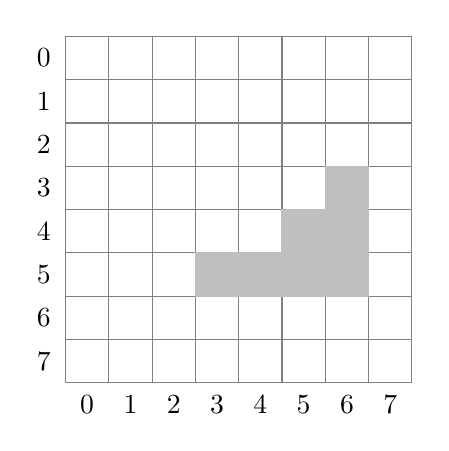
\begin{tikzpicture}[scale=1.1]
\draw[step=5mm,gray] (0,0) grid (4,4);
\foreach \r in {0,1,2,3,4,5,6,7}
  \node at (-.25,3.75-\r*.5) {$\r$};
\foreach \c in {0,1,2,3,4,5,6,7}
  \node at (.25+\c*.5,-.25) {$\c$};
\foreach \x/\y in {3/2, 4/2, 5/2, 6/2, 5/3, 6/3, 6/4}
   \draw[fill,gray!50] (\x/2,\y/2) rectangle +(5mm,5mm);
\path (4.1,0) -- (4.1,4.1); % Avoid truncation
\end{tikzpicture}
\caption{Carte discrète des cellules occupées d'un objet}\label{fig.disc}
\end{minipage}
\hspace{\fill}
\begin{minipage}{.45\textwidth}
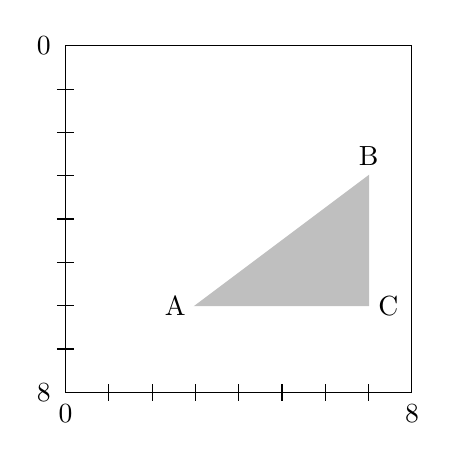
\begin{tikzpicture}[scale=1.1]
\draw (0,0) rectangle +(4,4);
\node at (-.25,0) {$8$};
\node at (-.25,4) {$0$};
\node at (0,-.25) {$0$};
\node at (4,-.25) {$8$};
\foreach \x in {1,2,3,4,5,6,7}
  \draw (\x*.5,-.1) -- (\x*.5,.1);
\foreach \y in {1,2,3,4,5,6,7}
  \draw (-.1,\y*.5) -- (.1,\y*.5);
\draw[fill,gray!50] (3/2,2/2) node[black,left] {\p{A}} -- (7/2,2/2) node[black,right] {\p{C}} -- (7/2,5/2) node[black,above] {\p{B}} -- cycle;
\path (4.1,0) -- (4.1,4.1); % Avoid truncation
\end{tikzpicture}
\caption{Une carte continue du même objet}
\label{fig.cont}
\end{minipage}
\end{figure}

La figure \ref{fig.cont} montre une \emph{carte continue}\index{map!continuous} du même objet. Au lieu de stocker les positions de l'objet, ce sont les coordonnées des positions des limites qui sont stockées :
\[
A = (6,3),\, B = (3,7),\, C = (6,7)\,.
\]

Les cartes discrètes ne sont pas très précises : il est difficile de reconnaître l'objet de la Fig.\ref{fig.disc} comme un triangle. Pour améliorer la précision, il faut utiliser une grille plus fine : 16$ fois 16$ ou même 256$ fois 256$. Bien entendu, plus le nombre de points de la grille augmente, plus la taille de la mémoire du robot doit être importante. En outre, un ordinateur plus puissant doit être utilisé pour traiter les cellules de la grille. Les robots mobiles sont soumis à des contraintes de poids, de coût, de capacité de batterie, etc. 

Si les objets de l'environnement sont peu nombreux et de forme simple, une carte continue est plus efficace et plus précise. Dans la figure \ref{fig.cont}, trois paires de nombres représentent le triangle avec beaucoup plus de précision que les sept paires de la carte discrète. En outre, il est facile de calculer si un point se trouve ou non dans l'objet à l'aide de la géométrie analytique. Cependant, s'il y a beaucoup d'objets ou s'ils ont des formes très complexes, les cartes continues ne sont plus efficaces, que ce soit en termes de mémoire ou de quantité de calculs nécessaires. L'objet de la Fig.~\ref{fig.cont} est délimité par des lignes droites, mais si la limite était décrite par des courbes d'ordre élevé, le calcul deviendrait difficile. Considérons une carte comportant $32$ objets de taille 1, dont aucun ne se touche. La carte discrète aurait $32$ coordonnées, tandis que la carte continue devrait stocker les coordonnées des quatre coins de chaque objet.

En robotique mobile, les cartes discrètes sont couramment utilisées pour représenter des cartes d'environnements, comme nous l'avons fait au chapitre \ref{ch.local}.

\section{Le contenu des cellules d'une carte en grille}\label{s.grids}
\index{cartographie!encodage}

Une carte géographique utilise des notations conventionnelles pour décrire l'environnement. Des couleurs sont utilisées : le vert pour les forêts, le bleu pour les lacs, le rouge pour les autoroutes. Des symboles sont utilisés : des points de différentes tailles pour indiquer les villages et les villes, et des lignes pour les routes, où l'épaisseur et la couleur d'une ligne sont utilisées pour indiquer la qualité de la route. Les robots utilisent des cartes quadrillées où chaque cellule stocke un nombre et nous devons décider ce qu'un nombre encode.

Le codage le plus simple consiste à attribuer un bit à chaque cellule. Une valeur de $1$ indique qu'un objet existe dans cette cellule et une valeur de $0$ indique que la cellule est vide. Dans la figure \ref{fig.disc}, le gris représente la valeur $1$ et le blanc la valeur $0$.

Cependant, les capteurs ne sont pas précis et il peut être difficile de savoir si une cellule est occupée par un objet ou non. Il est donc logique d'attribuer une probabilité à chaque cellule pour indiquer dans quelle mesure nous sommes certains que l'objet se trouve dans cette cellule. La figure \ref{fig.prob-grid} est une copie de la figure \ref{fig.disc} avec les probabilités énumérées pour chaque cellule. Les cellules sans numéro sont supposées avoir une probabilité de $0$.

\begin{figure}
\begin{center}
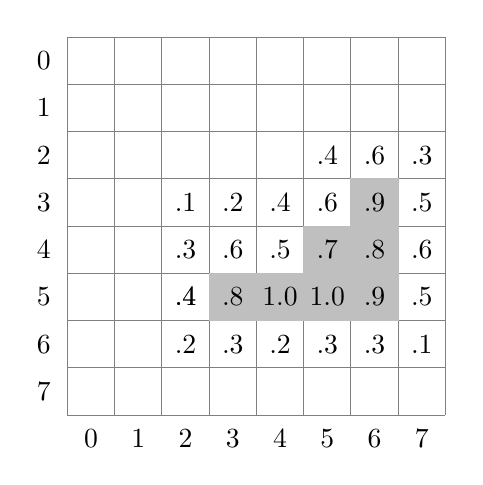
\begin{tikzpicture}[scale=1.2]
\draw[step=5mm,gray] (0,0) grid (4,4);
\foreach \r in {0,1,2,3,4,5,6,7}
  \node at (-.25,3.75-\r*.5) {$\r$};
\foreach \c in {0,1,2,3,4,5,6,7}
  \node at (.25+\c*.5,-.25) {$\c$};
\foreach \x/\y in {3/2, 4/2, 5/2, 6/2, 5/3, 6/3, 6/4}
   \draw[fill,gray!50] (\x/2,\y/2) rectangle +(5mm,5mm);
\foreach \x/\y/\p in {3/2/$.8$, 4/2/$1.0$, 5/2/$1.0$, 6/2/$.9$, 5/3/$.7$, 6/3/$.8$, 6/4/$.9$, 2/2/$.4$, 2/2/$.4$, 2/3/$.3$, 3/3/$.6$, 4/3/$.5$, 5/4/$.6$, 3/4/$.2$, 4/4/$.4$, 2/4/$.1$, 5/5/$.4$, 6/5/$.6$, 7/5/$.3$, 7/4/$.5$, 7/3/$.6$, 7/2/$.5$, 7/1/$.1$, 6/1/$.3$, 5/1/$.3$, 4/1/$.2$, 3/1/$.3$, 2/1/$.2$ }
   \node at (\x/2+.25,\y/2+.25) {\p};
\path (4.1,0) -- (4.1,4.1); % Avoid truncation
\end{tikzpicture}
\caption{Une carte de grille probabiliste}\label{fig.prob-grid}
\end{center}
\end{figure}

On constate que les cellules ayant une probabilité d'au moins $.7$ sont celles considérées dans la Fig.~\ref{fig.disc} comme étant des cellules occupées par l'objet. Bien entendu, nous sommes libres de choisir un autre seuil, par exemple $.5$, auquel cas davantage de cellules sont considérées comme occupées. Dans cet exemple, nous savons que l'objet est triangulaire, nous pouvons donc voir qu'un seuil de $.5$ rend l'objet plus grand qu'il ne l'est en réalité, alors que le seuil plus élevé de $.7$ donne une meilleure approximation.

\begin{framed}
\act{Carte probabiliste des obstacles}{carte des obstacles}
\begin{itemize}
\item Placez votre robot sur une ligne devant un ensemble d'obstacles que le robot peut détecter avec un capteur latéral (Fig.~\ref{fig.mapping-activity}). Si vous avez mis en œuvre la localisation comme décrit dans Activity~\ref{act.local-uncertain}, vous pouvez utiliser cette information pour établir où se trouve le robot. Sinon, dessinez des lignes régulières sur le sol qui peuvent être lues par le robot pour la localisation. Construisez une carte probabiliste des obstacles.
\item Comment les probabilités changent-elles lorsque des obstacles sont ajoutés ou supprimés ?
\end{itemize}
\end{framed}

\begin{figure}
\begin{center}
\begin{tikzpicture}
\draw[fill,lightgray] (-1,-2.5mm) rectangle +(8,5mm);
\pic[scale=1.2] at (0,-5mm) { robot2 };
\foreach \x in {-10mm, 5mm, 20mm, 35mm, 50mm, 65mm}
  \draw[fill,lightgray] (\x,-12mm) rectangle +(3mm,6mm);
\draw[fill] (5,1) rectangle +(12mm,5mm);
\draw[fill] (2,1) rectangle +(12mm,5mm);
\draw[dashed,thick] (15mm,4mm) -- +(20:10mm);
\draw[dashed,thick] (12mm,5mm) -- +(100:10mm);
\end{tikzpicture}
\end{center}
\caption{Les rectangles noirs représentent les obstacles à mesurer. La ligne grise guide le robot et les marques grises sont utilisées pour la localisation} \label{fig.mapping-activity}
\end{figure}

\section[L'algorithme de frontière]{Création d'une carte par exploration : L'algorithme de frontière} \label{s.map-create}
\index{cartographie!exploration de l'environnement}

Prenons l'exemple d'un aspirateur robotisé qui vient d'être lâché dans votre appartement. De toute évidence, il n'est pas préprogrammé avec une carte de votre appartement. Il doit donc explorer l'environnement pour recueillir des informations qui lui permettront de construire son propre plan. Il existe plusieurs façons d'explorer l'environnement, la plus simple étant l'exploration aléatoire. L'exploration sera beaucoup plus efficace si le robot dispose d'une carte partielle qu'il peut utiliser pour guider son exploration.

\subsection{Cartes en grille avec probabilités d'occupation}

La carte de la figure \ref{fig.map-explore} est une carte quadrillée où chaque cellule est étiquetée avec sa \emph{probabilité d'obstacle}\index{probabilité d'occupation de la carte}, qui est la probabilité qu'il y ait un obstacle dans la cellule. L'obstacle peut être un mur, une table ou toute autre chose qui ne permet pas au robot de passer par cette cellule. Les points d'interrogation représentent les cellules qui n'ont pas encore été explorées. En l'absence de toute connaissance sur le contenu d'une cellule, on peut supposer que la probabilité qu'il y ait un obstacle à cet endroit est de $0,5$, puisqu'elle peut tout aussi bien être occupée ou non. Un point d'interrogation est utilisé à la place de la valeur $0.5$ pour clarifier le statut inexploré des cellules.

\begin{figure}
\begin{center}
\includegraphics[width=\textwidth]{grid-mapping1.pdf}
\end{center}
\caption{Grid map of an environment with occupancy probabilities}\label{fig.map-explore}
\end{figure}

Le centre de la carte est libre de tout obstacle et les probabilités d'occupation de ces cellules, appelées "cellules ouvertes", sont faibles (0,1 $ ou 0,2 $). Il existe trois obstacles connus, en haut à droite, en haut à gauche et en bas au centre. Les obstacles sont caractérisés par des probabilités d'occupation élevées (0,9$ ou 1,0$) et sont indiqués par des cellules grises. Une cellule frontière est une cellule ouverte qui est adjacente (à gauche, à droite, en haut, en bas) à une ou plusieurs cellules inconnues. L'ensemble des cellules frontières est appelé \emph{frontière}. Les lignes rouges des petits carrés de la Fig.~\ref{fig.map-explore} représentent la limite entre la frontière et les cellules inconnues de l'environnement. Les cellules inconnues adjacentes à la frontière sont les cellules intéressantes qu'il convient d'explorer afin d'élargir la carte actuelle.

\subsection{L'algorithme de frontière}

L'algorithme \emph{frontière}\index{cartographie!algorithme frontière} est utilisé pour étendre la carte en explorant la frontière. Le robot se déplace jusqu'à la cellule frontière la plus proche, détecte s'il y a des obstacles dans les cellules adjacentes inconnues et met à jour la carte en conséquence. 

La carte de la grille de la figure \ref{fig.map-explore1} est la même que celle de la figure \ref{fig.map-explore} avec l'ajout du robot qui occupe une cellule colorée en bleu. La cellule frontière la plus proche du robot est la cellule située deux pas au-dessus de sa position initiale. La flèche indique que le robot s'est déplacé vers cette cellule. Le robot utilise ses capteurs locaux pour déterminer s'il y a des obstacles dans les cellules inconnues adjacentes. (Les capteurs peuvent détecter des obstacles dans les huit cellules adjacentes, y compris celles qui se trouvent sur la diagonale). Supposons que la cellule en haut à gauche contienne certainement un obstacle (probabilité $1.0$), alors que les cellules directement au-dessus et à droite ne contiennent presque certainement pas d'obstacle (probabilité $0.1$). La figure \ref{fig.map-explore2} montre la carte mise à jour avec ces nouvelles informations et la nouvelle position de la frontière.

\begin{figure}
\begin{center}
\includegraphics[width=\textwidth]{grid-mapping1b.pdf}
\end{center}
\caption{Le robot se déplace vers la frontière}\label{fig.map-explore1}
\end{figure}

\begin{figure}
\begin{center}
\includegraphics[width=\textwidth]{grid-mapping1c.pdf}
\end{center}
\caption{Le robot met à jour les cellules inconnues adjacentes à la frontière}
\label{fig.map-explore2}
\end{figure}

La figure \ref{fig.map-explore3} montre le résultat de l'itération suivante de l'algorithme. Le robot s'est déplacé d'une cellule vers la cellule frontière la plus proche, a détecté des obstacles dans les deux cellules inconnues adjacentes et a mis à jour la carte. L'obstacle en haut à droite est parfaitement connu et il n'y a pas de cellule frontière à proximité de la position actuelle du robot.

\begin{figure}
\begin{center}
\includegraphics[width=\textwidth]{grid-mapping1d.pdf}
\end{center}
\caption{Deuxième itération de l'algorithme de frontière}\label{fig.map-explore3}
\end{figure}

La figure~\ref{fig.map-explore4} montre l'itération suivante de l'algorithme. Le robot est bloqué par l'obstacle en haut à droite et doit l'éviter en se déplaçant vers la cellule frontière la plus proche.

La figure~\ref{fig.map-explore5} montre la carte complète construite par le robot après qu'il ait exploré toute la frontière, comme le montre le chemin avec les flèches bleues. 

L'algorithme~\ref{alg.frontier} formalise l'algorithme de frontière. Pour des raisons de simplicité, l'algorithme recalcule la frontière à chaque étape. Un algorithme plus sophistiqué examinerait les cellules dans le voisinage de la position du robot et ajouterait ou supprimerait les cellules dont le statut de cellule frontière a changé.

L'exemple auquel nous avons appliqué l'algorithme de frontière est un environnement relativement simple composé de deux pièces reliées par une porte (à la sixième colonne en partant de la gauche sur la Fig.~\ref{fig.map-explore5}), mais par ailleurs fermé à l'environnement extérieur. Cependant, l'algorithme de frontière fonctionne dans des environnements plus complexes. 

\begin{figure}
\begin{center}
\includegraphics[width=\textwidth]{grid-mapping1e.pdf}
\end{center}
\caption{Le robot évite un obstacle en se déplaçant vers la prochaine frontière}
\label{fig.map-explore4}
\end{figure}

\begin{figure}
\begin{center}
\includegraphics[width=\textwidth]{grid-mapping1f.pdf}
\end{center}
\caption{La carte construite par l'algorithme de frontière et le chemin exploré par le robot}
\label{fig.map-explore5}
\end{figure}

\begin{figure}
\begin{alg}{Algorithme de frontière}{frontier}
\hline
&\idv{}float array grid&// Grid map\\
&\idv{}cell list frontier&// List of frontier cells\\
&\idv{}cell robot& // Cell with robot\\
&\idv{}cell closest&// Closest cell to robot\\
&\idv{}cell c&// Index over cells\\
&\idv{}float low&// Low occupancy probability\\
\hline
\stl{}&loop&\\
\stl{}&\idc{}frontier \ass{} empty&\\
\stl{}&\idc{}for all known cells c  in the grid&\\
\stl{}&\idc{}\idc{}if grid(c) $<$ low and&\\
\stl{}&\idc{}\idc{}\idc{}exists unknown neighbor of c&\\
\stl{}&\idc{}\idc{}\idc{}\idc{}append c to frontier&\\
\stl{}&\idc{}exit if frontier empty&\\
&&\\
\stl{}&\idc{}closest \ass{} cell in frontier nearest robot&\\
\stl{}&\idc{}robot \ass{} closest&\\
\stl{}&\idc{}for all unknown neighbors c of closest&\\
\stl{}&\idc{}\idc{}\idc{}sense if c is occupied&\\
\stl{}&\idc{}\idc{}\idc{}mark grid(c)&\\
&\idc{}\idc{}\idc{}\idc{}with occupancy probability&\\
\end{alg}
\end{figure}

L'algorithme de frontière peut être exécuté en parallèle par plusieurs robots. Chaque robot explore la partie de la frontière la plus proche de sa position. Les robots partagent leurs cartes partielles afin de maintenir la cohérence des cartes. Comme chaque robot explore une zone différente de l'environnement, la construction de la carte sera beaucoup plus efficace.

\subsection{Priority in the frontier algorithm}\label{s.priority}

L'algorithme de frontière peut utiliser des critères autres que la distance pour choisir la frontière à explorer. Considérons l'exploration de la carte quadrillée présentée sur la Fig.~\ref{fig.map-seven}. Le robot se trouve dans la cellule $(3,3)$ marquée d'un cercle bleu. Il y a six cellules d'obstacles connues et cinq cellules ouvertes connues, dont les trois cellules $(1,3), (2,2), (3,2)$, marquées par des carrés rouges, sont les cellules frontières. (Ici, les voisins diagonaux ne sont pas considérés comme adjacents).

\begin{figure}
\begin{center}
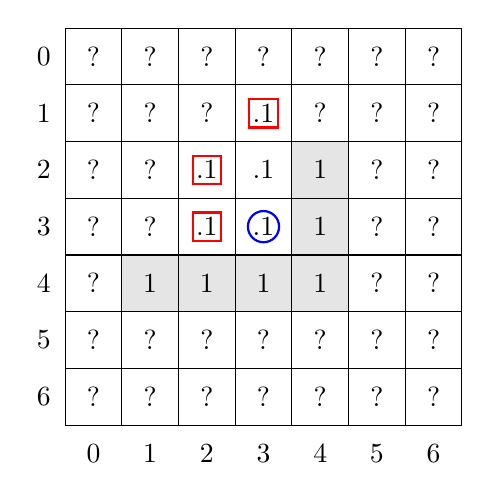
\begin{tikzpicture}[scale=.9]
% Obstacles
\foreach \r/\c in {32/32, 32/24, 32/16, 8/16, 16/16, 24/16}
  \fill[gray!20] (\r mm,\c mm) rectangle +(8mm,8mm);
% Robot
%\fill[gray!50] (24mm,24mm) rectangle +(8mm,8mm);
\draw[blue,thick] (28mm,28mm) circle [radius=2.2mm];
% Frontier
\foreach \r/\c in {18/26, 18/34, 26/42}
  \draw[red,thick] (\r mm,\c mm) rectangle +(4mm,4mm);
% Grid
\draw[step=8mm] (0,0) grid (56mm,56mm);
\foreach \r in {0,1,2,3,4,5,6} {
  \node at (\r*8mm+4mm,-4mm) {\p{\r}};
}
\foreach \r in {0,1,2,3,4,5,6} {
  \node at (-3mm,52mm-\r*8mm) {\p{\r}};
}
% Cells
\foreach \r in {0,1,2,3,4,5,6} {
  \node at (\r*8mm+4mm,52mm) {\p{?}};
}
\foreach \r/\a in {0/?,1/?,2/?,3/.1,4/?,5/?,6/?} {
  \node at (\r*8mm+4mm,44mm) {\p{\a}};
}
\foreach \r/\a in {0/?,1/?,2/.1,3/.1,4/1,5/?,6/?} {
  \node at (\r*8mm+4mm,36mm) {\p{\a}};
}
\foreach \r/\a in {0/?,1/?,2/.1,3/.1,4/1,5/?,6/?} {
  \node at (\r*8mm+4mm,28mm) {\p{\a}};
}
\foreach \r/\a in {0/?,1/1,2/1,3/1,4/1,5/?,6/?} {
  \node at (\r*8mm+4mm,20mm) {\p{\a}};
}
\foreach \r in {0,1,2,3,4,5,6} {
  \node at (\r*8mm+4mm,12mm) {\p{?}};
}
\foreach \r in {0,1,2,3,4,5,6} {
  \node at (\r*8mm+4mm,4mm) {\p{?}};
}
\end{tikzpicture}
\end{center}
\caption{Exploration d'un labyrinthe}
\label{fig.map-seven}
\end{figure}

Dans l'algorithme~\ref{alg.frontier}, le robot utilise la distance à une cellule frontière comme critère pour décider où se déplacer. Dans la figure \ref{fig.map-seven}, la cellule située à la gauche du robot à $(3,2)$ est la cellule la plus proche puisqu'elle n'est qu'à un pas, alors que les deux autres cellules frontières sont à deux pas. Nous pouvons considérer un critère différent en prenant en compte le nombre de cellules inconnues adjacentes à une cellule frontière. Commencer par une cellule frontière avec plus de cellules inconnues peut rendre l'algorithme plus efficace. Nous définissons la priorité d'une cellule frontière comme suit :
\[
p_\sub{cell} = \frac{a_\sub{cell}}{d_\sub{cell}}\,,
\]
où $a_\sub{cell}$ est le nombre de cellules inconnues adjacentes et $d_\sub{cell}$ est la distance par rapport au robot. Les priorités des trois cellules frontières sont les suivantes :
\[
p_{(3,2)} = 1/1 = 1,\;\;p_{(2,2)} = 2/2 = 1,\;\;p_{(1,3)} = 3/2 = 1.5\,.
\]
La priorité de la cellule $(1,3)$ est la plus élevée et l'exploration commence à cet endroit.

\begin{framed}
\act{algorithme de frontière}{frontière}
\begin{itemize}
\item Mettre en œuvre l'algorithme de frontière. Vous devrez inclure un algorithme permettant de se déplacer avec précision d'une cellule à l'autre et un algorithme permettant de contourner les obstacles.
\item Exécutez le programme sur la carte quadrillée de la Fig.~\ref{fig.map-explore5}. Obtenez-vous la même trajectoire ? Si ce n'est pas le cas, pourquoi ?
\item Exécuter le programme sur la carte quadrillée de la Fig.~\ref{fig.map-seven}.
\item Modifier l'Algorithme~\ref{alg.frontier} pour utiliser la priorité décrite dans Sect.~\ref{s.priority}. Le chemin est-il différent de celui généré par le programme original ?
\item Essayez d'implémenter l'algorithme de frontière sur votre robot. Quel est l'aspect le plus difficile de la mise en œuvre ?
\end{itemize}
\end{framed}

\section[La connaissance de l'environnement]{Cartographier en utilisant la connaissance de l'environnement}\label{s.map-update}
\index{cartographie!connaissance de l'environnement@{avec connaissance de l'environnement}}

Maintenant que nous savons comment explorer un environnement, examinons comment construire une carte pendant l'exploration. Au Chap.~\ref{ch.local}, nous avons vu qu'un robot peut se localiser à l'aide de repères externes et de leur représentation dans une carte. Sans ces repères externes, le robot ne peut compter que sur l'odométrie ou la mesure inertielle, qui sont sujettes à des erreurs qui augmentent avec le temps (Fig.~\ref{fig.odo-errors}). Comment est-il possible d'établir une carte lorsque la localisation est sujette à d'importantes erreurs ?

Même avec une mauvaise odométrie, le robot peut construire une meilleure carte s'il dispose d'informations sur la structure de l'environnement. Supposons que le robot essaie de construire le plan d'une pièce en suivant ses murs. Les différences entre les vitesses réelles des roues gauche et droite amèneront le robot à conclure que les murs ne sont pas droits (Fig.~\ref{fig.map-room1}), mais si le robot sait \emph{à l'avance} que les murs sont droits et perpendiculaires l'un à l'autre, il peut construire la carte montrée dans la Fig.~\ref{fig.map-room2}. Lorsqu'il rencontre un virage serré, il comprend qu'il s'agit d'un coin à $90^\circ$ où deux murs se rencontrent, et sa cartographie des angles sera donc correcte. Il y aura également une erreur lors de la mesure des longueurs des murs, ce qui peut entraîner l'écart illustré dans la figure entre le premier et le dernier mur. La figure montre un petit espace qui ne serait pas important, mais si le robot cartographie une grande zone, le problème de \emph{fermer une boucle}\index{simultaneous localization and mapping (SLAM)!fermer la boucle} dans une carte est difficile à résoudre parce que le robot n'a qu'une vue locale de l'environnement.

\begin{figure}
\begin{minipage}{.45\textwidth}
\begin{tikzpicture}[scale=1.2]
\pic[rotate=90,scale=.5] at (0,0) { robot };
\draw[bend right=10] (-6mm,0mm) to (-10mm,25mm);
\draw[bend right=10] (-10mm,25mm) to (10mm,35mm);
\draw[bend right=10] (10mm,35mm) to (25mm,20mm);
\draw[bend right=10] (25mm,20mm) to (20mm,5mm);
\end{tikzpicture}
\caption{Mouvement perçu d'un robot basé sur l'odométrie}
\label{fig.map-room1}
\end{minipage}
\hspace{\fill}
\begin{minipage}{.45\textwidth}
\begin{tikzpicture}[scale=1.2]
\pic[rotate=90,scale=.5] at (0,0) { robot };
\draw (-6mm,2mm)  to (-6mm,25mm);
\node at (-8mm,0mm) {\p{écart}};
\draw (-6mm,25mm) to (20mm,25mm);
\draw (20mm,25mm) to (20mm,-4mm);
\draw (20mm,-4mm) to (-6mm,-4mm);
\draw (-6mm,-4mm) to (-6mm,-2mm);
\end{tikzpicture}
\caption{Odométrie et connaissance de la géométrie des murs}
\label{fig.map-room2}
\end{minipage}
\end{figure}

Considérons une tondeuse à gazon robotisée à qui l'on confie la tâche de tondre une pelouse en se déplaçant d'avant en arrière ; elle doit fermer la boucle en retournant à sa station de charge (Fig.~\ref{fig.lawn}). Il n'est pas possible de mettre en œuvre ce comportement en utilisant uniquement l'odométrie, car de petites erreurs dans la vitesse et le cap entraînent de grandes erreurs dans la position du robot. Il est très peu probable que l'odométrie seule permette au robot de tondre toute la surface de la pelouse et de retourner à sa station de charge. Des points de repère tels que des câbles de signalisation dans le sol doivent être utilisés pour boucler la boucle.

\begin{figure}
\begin{center}
% Robotic lawnmower
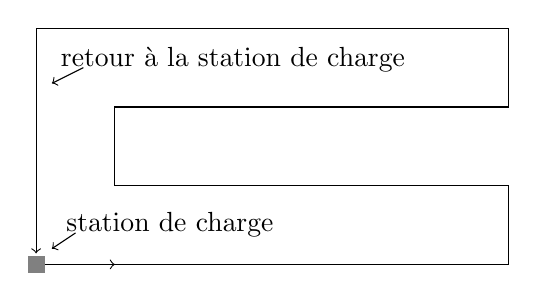
\begin{tikzpicture}[align=left]
\node at (2.5,2.6) {\p{retour à la station de charge}};
\draw[->] (.6,2.5) -- +(-4mm,-2mm);
\draw (0,0) -- (6,0) -- (6,1) -- (1,1) -- (1,2) -- (6,2) -- (6,3) -- (0,3);
\draw[->] (0,0) -- (1,0);
\draw[->] (0,3) -- (0,4pt);
\draw[fill,gray] (-1mm,-1mm) rectangle +(2mm,2mm);
\node at (1.7,.5) {\p{station de charge}};
\draw[->] (.5,.4) -- +(-3mm,-2mm);
\end{tikzpicture}
\end{center}
\caption{Une tondeuse à gazon robotisée tond une zone et retourne à sa station de charge.}
\label{fig.lawn}
\end{figure}

La construction de cartes peut être considérablement améliorée par l'utilisation de données de capteurs qui peuvent fournir des informations sur les caractéristiques régulières de l'environnement, en particulier à longue distance. Les caractéristiques régulières peuvent être des lignes au sol, une orientation globale ou la détection de caractéristiques qui \emph{overlap}\index{simultaneous localization and mapping (SLAM)!overlap} avec d'autres mesures. Supposons que nous disposions d'un capteur de distance capable de mesurer les distances sur une grande surface (Fig.~\ref{fig.map_overlap}). La mesure sur une grande surface permet au robot d'identifier des caractéristiques telles que les murs et les coins à partir d'une mesure prise à un seul endroit. Les mesures sur une grande surface facilitent l'identification des chevauchements entre les cartes locales qui sont construites à chaque endroit au fur et à mesure que le robot se déplace dans l'environnement. En comparant les cartes locales, la localisation peut être corrigée et la carte mise à jour avec précision. C'est le sujet de l'algorithme SLAM décrit dans la section suivante.

\begin{figure}
\begin{center}
\begin{tikzpicture}[scale=1.2]
\pic[rotate=90,scale=.5] at (0,0) { robot };
\pic[rotate=90,scale=.5] at (0,19mm) { robot };
\pic[scale=.5] at (10mm,28mm) { robot };
\draw[thick,dashed,color=red] (0,2mm) circle[radius=14mm];
\draw[thick,dashed,color=blue] (0,21mm) circle[radius=14mm];
\draw[thick,dashed,color=green!70!black] (12mm,28mm) circle[radius=14mm];
\draw[thick,color=red,yshift=-2pt] (-6mm,-10mm) -- (-6mm,15mm);
\draw[thick,color=blue] (-7mm,9mm) -- (-7mm,33mm) -- (8mm,33mm);
\draw[thick,color=green!70!black] (-1mm,34mm) -- (25mm,34mm);
\end{tikzpicture}
\end{center}
\caption{Les mesures des capteurs à longue portée permettent de détecter les chevauchements}
\label{fig.map_overlap}
\end{figure}

\begin{framed}
\act{Tondeuse à gazon robotisée}{}%{Tondeuse à gazon}
\begin{itemize}
\item Écrire un programme qui permet à une tondeuse à gazon robotisée de se déplacer le long d'une trajectoire en utilisant uniquement l'odométrie (Fig.~\ref{fig.lawn}). Exécutez le programme plusieurs fois. Le robot revient-il à la station de charge ? Si ce n'est pas le cas, quelle est l'ampleur des erreurs ? Les erreurs sont-elles constantes ou changent-elles d'une exécution à l'autre ?
\item Placez des points de repère avec du ruban adhésif noir autour de la pelouse (Fig.~\ref{fig.lawn-landmarks}). Programmez votre robot pour qu'il reconnaisse les repères et corrige sa localisation. Quelle doit être la taille des repères pour que le robot les détecte de manière fiable ?
\end{itemize}
\end{framed}

\begin{figure}
\begin{center}
% Robotic lawnmower with landmarks
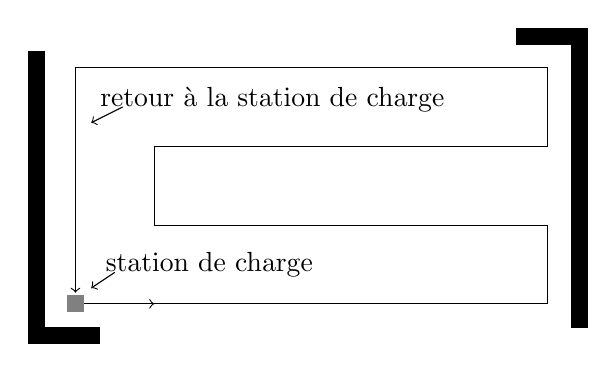
\begin{tikzpicture}[align=left]
\node at (2.5,2.6) {\p{retour à la station de charge}};
\draw[->] (.6,2.5) -- +(-4mm,-2mm);
\draw (0,0) -- (6,0) -- (6,1) -- (1,1) -- (1,2) -- (6,2) -- (6,3) -- (0,3);
\draw[->] (0,0) -- (1,0);
\draw[->] (0,3) -- (0,4pt);
\draw[fill,gray] (-1mm,-1mm) rectangle +(2mm,2mm);
\node at (1.7,.5) {\p{station de charge}};
\draw[->] (.5,.4) -- +(-3mm,-2mm);
\draw[fill,black] (-.6,-.4) rectangle +(2mm,3.6);
\draw[fill,black] (-.6,-.5) rectangle +(9mm,2mm);
\draw[fill,black] (6.3,-.3) rectangle +(2mm,3.6);
\draw[fill,black] (6.5,3.3) rectangle +(-9mm,2mm);
\end{tikzpicture}
\end{center}
\caption{Une tondeuse robotisée avec des points de repère}
\label{fig.lawn-landmarks}
\end{figure}

\section{Exemple numérique d'un algorithme SLAM}\label{s.slam-numerical}
\index{localisation et cartographie simultanées (SLAM)!exemple numérique}

L'algorithme SLAM est assez compliqué, c'est pourquoi nous calculons d'abord un exemple numérique avant d'en donner la présentation formelle.

La figure~\ref{fig.mapping1a} montre un robot dans une pièce se dirigeant vers le haut du diagramme. Le robot se trouve près d'un coin de la pièce et il y a une projection du mur à la gauche du robot, peut-être un pilier de soutien du bâtiment. La Fig.~\ref{fig.mapping1b} est la carte correspondante. Le gros point indique la position du robot et la flèche associée indique sa direction. La ligne pointillée épaisse représente le mur réel. Les cellules blanches représentent les endroits connus pour être libres, les cellules grises représentent les obstacles, et les cellules avec des points d'interrogation sont encore inexplorées. Une cellule est considérée comme faisant partie de l'obstacle si la majorité de sa surface se trouve derrière le mur. Par exemple, les deux segments horizontaux de la projection à partir du mur sont proches de la limite des cellules qu'ils traversent, mais ces cellules sont considérées comme faisant partie de l'obstacle parce que la quasi-totalité de leur surface se trouve derrière le mur.

\begin{figure}
\begin{minipage}{.45\textwidth}
\includegraphics[width=.4\textwidth]{mappingA.pdf}
\caption{Un robot près du mur d'une pièce}
\label{fig.mapping1a}
\end{minipage}
\hspace{\fill}
\begin{minipage}{.45\textwidth}
\includegraphics[width=.4\textwidth]{mappingB.pdf}
\caption{La carte correspondante}
\label{fig.mapping1b}
\end{minipage}
\end{figure}

Pour présenter les détails de l'algorithme SLAM, la carte est fortement simplifiée. Tout d'abord, les cellules sont beaucoup trop grandes, à peu près de la même taille que le robot lui-même. En pratique, les cellules seraient beaucoup plus petites que le robot. Deuxièmement, nous spécifions que chaque cellule (explorée) est soit libre (blanche), soit contient un obstacle (grise) ; les vrais algorithmes SLAM utilisent une représentation probabiliste (Sect.~\ref{s.grids}).

Supposons que le robot de la Fig.~\ref{fig.mapping1a} ait l'intention de se déplacer vers l'avant jusqu'à la nouvelle position indiquée sur la Fig.~\ref{fig.mapping2a}. La figure~\ref{fig.mapping2b} montre la carte correspondant à la position après le déplacement prévu, où le robot s'est déplacé de la hauteur d'une cellule vers le haut par rapport à sa position initiale. Malheureusement, la roue droite se déplace sur une zone de faible friction et, bien que le robot se retrouve à la bonne position, son cap est trop à droite. La position réelle du robot est représentée sur la Fig.~\ref{fig.mapping2c} et la Fig.~\ref{fig.mapping2d} est la carte correspondante.

\begin{figure}
\begin{minipage}{.45\textwidth}
\includegraphics[width=.43\textwidth]{mapping2A.pdf}
\caption{Le mouvement prévu du robot}
\label{fig.mapping2a}
\end{minipage}
\hspace{\fill}
\begin{minipage}{.45\textwidth}
\includegraphics[width=.43\textwidth]{mapping2B.pdf}
\caption{La carte du mouvement prévu}
\label{fig.mapping2b}
\end{minipage}
\end{figure}

\begin{figure}
\begin{minipage}{.45\textwidth}
\includegraphics[width=.43\textwidth]{mapping2C.pdf}
\caption{Le mouvement réel du robot}
\label{fig.mapping2c}
\end{minipage}
\hspace{\fill}
\begin{minipage}{.45\textwidth}
\includegraphics[width=.43\textwidth]{mapping2D.pdf}
\caption{La carte du mouvement réel}
\label{fig.mapping2d}
\end{minipage}
\end{figure}

La figure \ref{fig.mapping3a} (qui est la même que la figure \ref{fig.mapping2b}) montre la perception \emph{intended} du robot parce que le robot s'est déplacé d'une cellule vers le haut par rapport à la carte de la figure \ref{fig.mapping1b}. Dans cette position, il peut détecter l'obstacle à sa gauche et examiner les cellules inconnues devant lui.

Cependant, en raison de l'erreur d'odométrie, la perception \emph{actuelle} du robot est différente. La figure \ref{fig.mapping3b} montre la position réelle du mur telle qu'elle est vue par le robot, superposée aux cellules, où les cellules sont colorées en gris si l'on sait que la majorité de leur zone se trouve derrière le mur. (Nous supposons que le robot peut détecter les murs à une distance allant jusqu'à cinq fois la taille d'une cellule, comme le montre le cercle en pointillé, et nous supposons également que le robot sait que tout mur a une épaisseur d'une cellule.

\begin{figure}
\begin{minipage}{.45\textwidth}
\includegraphics[width=.43\textwidth]{mapping3A.pdf}
\caption{La perception prévue du robot}
\label{fig.mapping3a}
\end{minipage}
\hspace{\fill}
\begin{minipage}{.45\textwidth}
\includegraphics[width=.43\textwidth]{mapping3B.pdf}
\caption{La perception réelle du robot}
\label{fig.mapping3b}
\end{minipage}
\end{figure}

Il y a un décalage évident entre la carte actuelle et les données du capteur qui devraient correspondre à la partie connue de la carte. De toute évidence, le robot ne se trouve pas à l'endroit où il devrait être d'après l'odométrie. Comment ce décalage peut-il être corrigé ? Nous supposons que l'odométrie donne une estimation raisonnable de la pose (position et cap) du robot. Pour chaque erreur possible relativement faible dans la pose, nous calculons ce que serait la perception de la carte actuelle et la comparons à la perception réelle calculée à partir des données du capteur. La pose qui donne la meilleure correspondance est choisie comme la pose réelle du robot et la carte actuelle est mise à jour en conséquence.

Dans l'exemple, on suppose que le robot se trouve soit dans la cellule attendue, soit dans l'une de ses quatre cellules voisines (gauche, droite, haut, bas) et que le cap du robot est soit correct, soit légèrement tourné vers la droite ($15^\circ$ dans le sens des aiguilles d'une montre (CW)) ou légèrement tourné vers la gauche ($15^\circ$ dans le sens inverse des aiguilles d'une montre (CCW)). Les $5\times 3=15$ poses possibles sont illustrées dans la Fig.~\ref{fig.pos-explore} et la Fig.~\ref{fig.mapping4} montre la perception de la carte calculée à partir de la carte actuelle pour chaque pose. (Pour gagner de la place, seul un fragment de $8\times 5$ de la carte de $12\times 8$ est affiché).

\begin{figure}
\begin{center}
\includegraphics[width=0.5\textwidth]{pos-explore.pdf}
\end{center}
\caption{Positions possibles du robot}
\label{fig.pos-explore}
\end{figure}

\begin{figure}
\begin{center}
\includegraphics[width=0.9\textwidth]{mapping4b.pdf}
\end{center}
\caption{Estimations de la perception du robot pour différentes poses}
\label{fig.mapping4}
\end{figure}

L'étape suivante consiste à choisir la carte qui correspond le mieux aux mesures du capteur. Transformons d'abord les cartes $8\times 5$ en matrices $8\times 5$, en attribuant $-1$ aux cellules vides, $+1$ aux cellules d'obstacles et $0$ aux autres cellules. La matrice de gauche de la figure \ref{fig.mapping5} est associée à la carte actuelle et la matrice centrale de la figure est associée à la carte de perception correspondant à la pose où le robot est dans la cellule correcte mais le cap est $15^circ$ CW (l'élément central de la rangée supérieure de la figure \ref{fig.mapping4}).

Pour comparer les cartes, multipliez les éléments des cellules correspondantes. Soit $m(i,j)$ la $(i,j)$'th cell de la carte actuelle et $p(i,j)$ la $(i,j)$'th cell de la carte de perception obtenue à partir des valeurs des capteurs. $S(i,j)$, l'\emph{similarité} de la $(i,j)$ ème cellule, est :
\[
S(i,j) = m(i,j)\, p(i,j)\,,
\]
qui peut également être exprimée comme suit
\[
\begin{array}{l@{\hspace{2em}}l}
S(i,j) = 1 & \textrm{if}\;\;m(i,j) \neq 0,\, p(i,j) \neq 0,\, m(i,j) = p(i,j)\\
S(i,j) = -1 & \textrm{if}\;\;m(i,j) \neq 0,\, p(i,j) \neq 0,\,  m(i,j) \neq p(i,j)\\
S(i,j) = 0 & \textrm{if }m(i,j) = 0\, \textrm{or}\; p(i,j) = 0\,.
\end{array}
\]
La matrice de droite dans la Fig.\ref{fig.mapping5} montre le résultat de ce calcul pour les deux matrices à sa gauche. Il y a beaucoup de $1$, ce qui signifie que les matrices sont similaires et que nous pouvons donc conclure que les cartes de perception sont similaires. Pour obtenir un résultat quantitatif, calculez la somme des similitudes afin d'obtenir une valeur unique pour toute paire $m,p$ :
\[
\mathcal{S} = \sum_{i=1}^8 \sum_{j=1}^5 S(i,j)\,.
\]

\begin{figure}
\begin{center}
\includegraphics[width=\textwidth]{mapping5.pdf}
\end{center}
\caption{Calcul de la correspondance entre deux cartes}
\label{fig.mapping5}
\end{figure}

Le tableau~\ref{tab.matching} donne les valeurs de la similarité $\mathcal{S}$ pour toutes les cartes de perception de la Fig.~\ref{fig.mapping4} par rapport à la carte actuelle. Comme prévu, la similarité la plus élevée est obtenue pour la carte correspondant à la pose avec la position correcte et le cap tourné de $15^\circ$ CW.

\begin{table}
\caption{Similarité $\mathcal{S}$ de la carte basée sur le capteur avec la carte actuelle}
\label{tab.matching}
\renewcommand{\arraystretch}{1.2}
\setlength{\tabcolsep}{8pt}
\begin{tabular}{p{33mm}ccc}
\hline
&Orientation prévue&$15^{\circ}$ CW&$15^{\circ}$ CCW\\
Position prévue & $22$ & \boldmath $32$ & $20$\\
Remonter d'une cellule & $23$ & $25$ & $16$\\
En bas d'une cellule     & $19$ & $28$ & $21$\\
Gauche d'une cellule     & $6$  & $7$  & $18$\\
Une cellule à droite    & $22$ & $18$ & $18$\\
\hline
\end{tabular}
\end{table}

Une fois ce résultat obtenu, nous corrigeons la pose du robot et utilisons les données de la carte de perception pour mettre à jour la carte actuelle stockée dans la mémoire du robot (Fig.~\ref{fig.final-map}).

\begin{figure}
\begin{center}
\includegraphics[width=\textwidth]{final-map.pdf}
\end{center}
\caption{Carte avant et après la mise à jour en utilisant les données de la carte de perception}
\label{fig.final-map}
\end{figure}

\section{Activités de démonstration de l'algorithme SLAM}\label{s.slam-activities}

Les deux activités suivantes démontrent certains aspects de l'algorithme SLAM. L'activité~\ref{act.computed-perceptions} suit l'algorithme et est destinée à être mise en œuvre dans un logiciel. L'activité~\ref{act.measured-perceptions} démontre un élément clé de l'algorithme qui peut être mis en œuvre sur un robot éducatif.

Les activités sont basées sur la configuration présentée dans la Fig.~\ref{fig.slam-config}. Le robot est situé à l'origine du système de coordonnées avec la pose $((x,y),\theta)=((0,0),0^\circ)$.\footnote{Il est pratique de prendre le cap du robot comme $0^\circ$.} Compte tenu de l'incertitude de l'odométrie, le robot peut en fait être situé à n'importe laquelle des coordonnées $(-1,0), (1,0), (0,-1), (0,1)$ et son orientation peut être $-15^\circ, 0, -15^\circ$ (comme le montrent les flèches en pointillés), ce qui donne $15$ poses possibles. Les trois points gris aux coordonnées $(2,2), (2,0), (2,-2)$ représentent des obstacles connus sur la carte actuelle. (Pour gagner de la place, les points sont affichés aux coordonnées $(2,1), (2,0), (2,-1)$). Les obstacles peuvent être détectés par plusieurs capteurs de proximité horizontaux, mais pour les besoins des activités, nous spécifions qu'il y a trois capteurs.

\begin{figure}
\begin{center}
% SLAM algorithm
\begin{tikzpicture}
\draw[step=3cm,very thin,gray] (-3.01,-3.01) grid (6,3);
% The obstacles
\fill[gray!80!black] (6,0) circle[radius=6pt];
\fill[gray!80!black] (6,3) circle[radius=6pt];
\fill[gray!80!black] (6,-3) circle[radius=6pt];
% The robots
\pic at (0,0) { robot };
\pic at (3,0) { robot };
\pic at (-3,0) { robot };
\pic at (0,3) { robot };
\pic at (0,-3) { robot };
% The three arrows on each robot
\foreach \x/\y in {0/0, 3/0, -3/0, 0/3, 0/-3} {
  \draw[dashed,->,thick] (\x,\y) -- +( 20:15mm);
  \draw[dashed,->,thick] (\x,\y) -- +(  0:15mm);
  \draw[dashed,->,thick] (\x,\y) -- +(-20:15mm);
}
\node at (-3.6,-2.9) {$(-1,-1)$};
\node at (3,3.3) {$(1,1)$};
\end{tikzpicture}
\caption{Configuration de l'algorithme SLAM}
\label{fig.slam-config}
\end{center}
\end{figure}

Dans l'algorithme SLAM, la "perception" d'un obstacle est la valeur renvoyée par un capteur de distance. Pour éviter d'avoir à définir un modèle pour les capteurs, les activités définiront une perception comme étant la \emph{distance} et la \emph{orientation} entre le capteur et l'obstacle.

\begin{framed}
\act{Localiser le robot à partir des perceptions calculées}{computed-perceptions}
\begin{itemize}
\item Pour chacune des $15$ positions, calculer l'ensemble des perceptions de chaque obstacle. Par exemple, si le robot se trouve à la position $((0.0,1.0),-15.0^\circ)$, l'ensemble des perceptions des trois obstacles est :
\[
[( 2.2,  41.6^\circ),\,  ( 2.2, -11.6^\circ),\,  ( 3.6, -41.3^\circ)]\,.
\]
\item Étant donné un ensemble de perceptions mesurées, calculer leurs similitudes avec les perceptions des $15$ poses du robot. Choisir la pose ayant la meilleure similarité comme étant la pose réelle du robot. Par exemple, pour l'ensemble des perceptions mesurées :
\[
[( 2.0,  32.0^\circ),\,  ( 2.6, -20.0^\circ),\,  ( 3.0, -30.0^\circ)]\,,
\]
et la similarité calculée comme la somme des différences absolues des éléments des perceptions, la pose avec la meilleure similarité est $((0.0, 1.0),-15.0^\circ)$.
\item Expérimenter avec différentes fonctions de similarité.
\item Nous avons calculé que la pose du robot est approximativement $((0.0, 1.0),-15.0^\circ)$. Supposons qu'un nouvel obstacle soit placé aux coordonnées $(3,0)$. Calculer la perception $(d,\theta)$ de l'objet à partir de cette pose, puis calculer la coordonnée $(x,y)$ du nouvel obstacle. Le nouvel obstacle peut être ajouté à la carte avec cette coordonnée.
\item La coordonnée calculée est-elle significativement différente de la coordonnée $(3,0)$ qui serait obtenue si le robot se trouvait à la position prévue $((0,0),0^\circ)$ ?
\end{itemize}
\end{framed}

\begin{framed}
\act{Localiser le robot à partir des perceptions mesurées}{measured-perceptions}
\begin{itemize}
\item Placer trois objets comme indiqué sur la Fig.~\ref{fig.slam-config}.
\item Écrire un programme qui mémorise l'ensemble des valeurs renvoyées par les trois capteurs de proximité horizontaux. Placez votre robot successivement dans chacune des $15$ positions et enregistrez les ensembles de valeurs. Vous disposez maintenant d'une base de données de perceptions : un ensemble de trois lectures de capteurs pour chaque pose.
\item Placez le robot dans l'une des positions et enregistrez l'ensemble des valeurs renvoyées par les capteurs. Calculez la similarité de cet ensemble avec chacun des ensembles de la base de données. Afficher la position associée à la meilleure similarité.
\item Expérimentez en plaçant le robot dans différentes positions et plusieurs fois dans chaque position. Quelle est la précision de la détermination de la pose ?
\item Expérimenter avec différentes fonctions de similarité.
\end{itemize}
\end{framed}

\section{La formalisation de l'algorithme SLAM}\label{s.slam-formal}
\index{algorithme de localisation et de cartographie simultanées (SLAM)!}

L'algorithme~\ref{alg.slam} est un algorithme SLAM qui trouve la position dont la carte de perception est la plus proche de la carte de perception obtenue à partir des données des capteurs. Le robot est localisé à cette position et la carte est mise à jour en fonction de ce qui est perçu à cette position.

\begin{figure}
\begin{alg}{SLAM}{slam}
\hline
&\idv{}matrix $\vec{m}$ \ass partial map&// Current map\\
&\idv{}matrix $\vec{p}$&// Perception map\\
&\idv{}matrix $\vec{e}$&// Expected map\\
&\idv{}coordinate $\vec{c}$ \ass initial position&// Current position\\
&\idv{}coordinate $\vec{n}$&// New position\\
&\idv{}coordinate array $\vec{T}$&// Set of test positions\\
&\idv{}coordinate $\vec{t}$&// Test position\\
&\idv{}coordinate $\vec{b}$ \ass none&// Best position\\
\hline
\stl{}&loop&\\
\stl{}&\idc{}move a short distance&\\
\stl{}&\idc{}$\vec{n}$ \ass odometry($\vec{c}$)&// New position\\
&&\hspace{2em} based on odometry\\
\stl{}&\idc{}$\vec{p}$ \ass analyze sensor data&\\
&&\\
\stl{}&\idc{}for every $\vec{t}$ in $\vec{T}$&// T is the positions around n\\
\stl{}&\idc{}\idc{}$\vec{e}$ \ass expected($\vec{m}$, $\vec{t}$)&// Expected map at test position\\
\stl{}&\idc{}\idc{}if compare($\vec{t}$,$\vec{e}$) better than $\vec{b}$&\\
\stl{}&\idc{}\idc{}\idc{}$\vec{b}$ \ass $\vec{t}$&// Best test position so far\\
&&\\
\stl{}&\idc{}$\vec{n}$ \ass $\vec{b}$&// Replace new position\\
&&\hspace{2em} by best position\\
\stl{}&\idc{}$\vec{m}$ \ass update($\vec{m}$,$\vec{p}$,$\vec{n})$&// Update map\\
&&//\hspace{2em}based on new position\\
\stl{}&\idc{}$\vec{c}$ \ass $\vec{n}$&// Current position is new position\\
\end{alg}
\end{figure}

L'algorithme est divisé en trois phases. Dans la première phase (lignes~2--4), le robot se déplace sur une courte distance et sa nouvelle position est calculée par odométrie. La carte de perception à cet endroit est obtenue en analysant les données des capteurs.

En supposant que l'erreur d'odométrie est relativement faible, nous pouvons définir un ensemble de positions de test où le robot pourrait se trouver. Dans la deuxième phase (lignes~5--8), la carte attendue à chacune de ces positions est calculée et comparée à la carte actuelle. La meilleure correspondance est sauvegardée.

Dans la troisième phase (lignes~9--11), la position avec la meilleure correspondance devient la nouvelle position et la carte actuelle est mise à jour en conséquence.

En pratique, l'algorithme est un peu plus compliqué car il doit tenir compte du fait que la carte de perception obtenue à partir des capteurs est limitée par la portée de ces derniers. Le chevauchement sera partiel à la fois parce que la portée des capteurs ne couvre pas la totalité de la carte actuelle et parce que les capteurs peuvent détecter des obstacles et des zones libres en dehors de la carte actuelle. Par conséquent, la taille de la carte perçue $\vec{p}$ sera beaucoup plus petite que la carte attendue $\vec{e}$ et la fonction \p{compare(}$\vec{p}$\p{,}$\vec{e}$\p{)} ne comparera que les zones qui se chevauchent. En outre, lors de la mise à jour de la carte actuelle, les zones qui n'y figuraient pas auparavant seront ajoutées. Sur la figure \ref{fig.final-map}, certaines cellules de la carte actuelle se trouvent en dehors du rayon de cinq cellules du capteur et ne seront pas mises à jour. Les cellules rouge clair étaient inconnues dans la carte actuelle, comme l'indiquent les points d'interrogation, mais dans la carte de perception, on sait maintenant qu'elles font partie de l'obstacle. Cette information est utilisée pour mettre à jour la carte actuelle afin d'obtenir une nouvelle carte actuelle.

\section{Résumé}

Un mouvement robotique précis dans un environnement incertain exige que le robot dispose d'une carte de l'environnement. La carte doit être conservée dans l'ordinateur du robot ; il peut s'agir d'une grille de cellules ou d'une représentation graphique d'une carte continue. Dans un environnement incertain, le robot ne dispose généralement pas d'une carte avant de commencer ses tâches. L'algorithme de frontière est utilisé par un robot pour construire une carte au fur et à mesure qu'il explore son environnement. Des cartes plus précises peuvent être construites si le robot a une certaine connaissance de son environnement, par exemple s'il sait qu'il s'agit de l'intérieur d'un bâtiment composé de pièces rectangulaires et de couloirs. Les algorithmes de localisation et de cartographie simultanées (SLAM) utilisent un processus itératif pour construire une carte tout en corrigeant les erreurs de localisation.

\section{Lecture complémentaire}

Deux manuels sur la planification des trajectoires et des mouvements sont \cite{latombe,lavalle}. Voir également \cite[Chapitre 6]{siegwart}.

L'algorithme de frontière a été proposé par Yamauchi \cite{yamauchi} qui a montré qu'un robot pouvait utiliser l'algorithme pour explorer avec succès un bureau avec des obstacles.

Les algorithmes de SLAM utilisent les probabilités, en particulier la règle de Bayes. Les méthodes probabilistes en robotique font l'objet du manuel \cite{thrun}.

Un tutoriel en deux parties sur le SLAM, rédigé par Durrant-Whyte et Bailey, est disponible dans \cite{slam-tutorial1,slam-tutorial2}. Un tutoriel sur la SLAM basée sur les graphes est disponible dans \cite{slam-graph}.

Le cours en ligne de Sebastian Thrun \emph{Artificial Intelligence for Robotics} est utile : \par\url{https://classroom.udacity.com/courses/cs373}.

